\begin{figure}[h]
\begin{minipage}{0.30\textwidth}
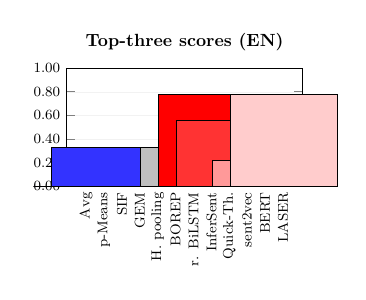
\begin{tikzpicture}[scale=0.75,every node/.style={scale=0.85}]
	\begin{axis}[
    		title=\textbf{Top-three scores (EN)},
		scale only axis,
		clip=false,
		separate axis lines,
		xtick={1,2,3,4,5,6,7,8,9,10,11,12},
        	x tick style={draw=none},
        	xticklabels={Avg,p-Means,SIF,GEM,H. pooling,BOREP,r. BiLSTM,InferSent,Quick-Th.,sent2vec,BERT,LASER},
		width=4cm,height=2cm,
		tick label style={font=\footnotesize},
		xticklabel style={rotate=90},
		ymajorgrids,
    		grid style={line width=.1pt, draw=gray!10},
		ymin=0,ymax=1,
		every axis plot/.append style={
          		ybar,
          		bar width=6.0,
          		bar shift=0.5pt,
			fill
		},
		scaled y ticks=false,
		y tick label style={
        		/pgf/number format/.cd,
            		fixed,
            		fixed zerofill,
            		precision=2,
        		/tikz/.cd
    		}
	]

		\addplot[draw=black,fill=blue] coordinates {(1,0.00)};
     	 	\addplot[draw=black,fill=blue!80] coordinates {(2,0.33)};
      		\addplot[draw=black,fill=blue!60] coordinates {(3,0.00)};
      		\addplot[draw=black,fill=blue!40] coordinates {(4,0.00)};
		\addplot[draw=black,fill=blue!20] coordinates {(5,0.00)};
     	 	\addplot[draw=black,fill=gray] coordinates {(6,0.00)};
      		\addplot[draw=black,fill=lightgray] coordinates {(7,0.33)};
      		\addplot[draw=black,fill=red] coordinates {(8,0.78)};
     	 	\addplot[draw=black,fill=red!80] coordinates {(9,0.56)};
      		\addplot[draw=black,fill=red!60] coordinates {(10,0.00)};
      		\addplot[draw=black,fill=red!40] coordinates {(11,0.22)};
		\addplot[draw=black,fill=red!20] coordinates {(12,0.78)};
	\end{axis}
\end{tikzpicture}
\end{minipage}
\hfill
\begin{minipage}{0.30\textwidth}
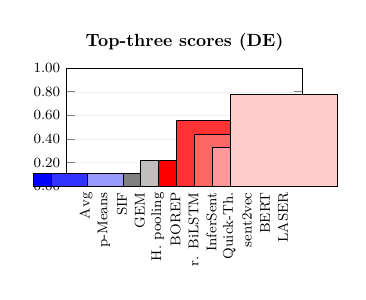
\begin{tikzpicture}[scale=0.75,every node/.style={scale=0.85}]
	\begin{axis}[
    		title=\textbf{Top-three scores (DE)},
		scale only axis,
		clip=false,
		separate axis lines,
		xtick={1,2,3,4,5,6,7,8,9,10,11,12},
        	x tick style={draw=none},
        	xticklabels={Avg,p-Means,SIF,GEM,H. pooling,BOREP,r. BiLSTM,InferSent,Quick-Th.,sent2vec,BERT,LASER},
		width=4cm,height=2cm,
		tick label style={font=\footnotesize},
		xticklabel style={rotate=90},
		ymajorgrids,
    		grid style={line width=.1pt, draw=gray!10},
		ymin=0,ymax=1,
		every axis plot/.append style={
          		ybar,
          		bar width=6.0,
          		bar shift=0.5pt,
			fill
		},
		scaled y ticks=false,
		y tick label style={
        		/pgf/number format/.cd,
            		fixed,
            		fixed zerofill,
            		precision=2,
        		/tikz/.cd
    		}
	]

		\addplot[draw=black,fill=blue] coordinates {(1,0.11)};
     	 	\addplot[draw=black,fill=blue!80] coordinates {(2,0.11)};
      		\addplot[draw=black,fill=blue!60] coordinates {(3,0.00)};
      		\addplot[draw=black,fill=blue!40] coordinates {(4,0.11)};
		\addplot[draw=black,fill=blue!20] coordinates {(5,0.00)};
     	 	\addplot[draw=black,fill=gray] coordinates {(6,0.11)};
      		\addplot[draw=black,fill=lightgray] coordinates {(7,0.22)};
      		\addplot[draw=black,fill=red] coordinates {(8,0.22)};
     	 	\addplot[draw=black,fill=red!80] coordinates {(9,0.56)};
      		\addplot[draw=black,fill=red!60] coordinates {(10,0.44)};
      		\addplot[draw=black,fill=red!40] coordinates {(11,0.33)};
		\addplot[draw=black,fill=red!20] coordinates {(12,0.78)};
	\end{axis}
\end{tikzpicture}
\end{minipage}
\hfill
\begin{minipage}{0.30\textwidth}
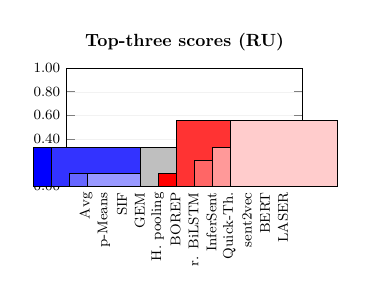
\begin{tikzpicture}[scale=0.75,every node/.style={scale=0.85}]
	\begin{axis}[
    		title=\textbf{Top-three scores (RU)},
		scale only axis,
		clip=false,
		separate axis lines,
		xtick={1,2,3,4,5,6,7,8,9,10,11,12},
        	x tick style={draw=none},
        	xticklabels={Avg,p-Means,SIF,GEM,H. pooling,BOREP,r. BiLSTM,InferSent,Quick-Th.,sent2vec,BERT,LASER},
		width=4cm,height=2cm,
		tick label style={font=\footnotesize},
		xticklabel style={rotate=90},
		ymajorgrids,
    		grid style={line width=.1pt, draw=gray!10},
		ymin=0,ymax=1,
		every axis plot/.append style={
          		ybar,
          		bar width=6.0,
          		bar shift=0.5pt,
			fill
		},
		scaled y ticks=false,
		y tick label style={
        		/pgf/number format/.cd,
            		fixed,
            		fixed zerofill,
            		precision=2,
        		/tikz/.cd
    		}
	]

		\addplot[draw=black,fill=blue] coordinates {(1,0.33)};
     	 	\addplot[draw=black,fill=blue!80] coordinates {(2,0.33)};
      		\addplot[draw=black,fill=blue!60] coordinates {(3,0.11)};
      		\addplot[draw=black,fill=blue!40] coordinates {(4,0.11)};
		\addplot[draw=black,fill=blue!20] coordinates {(5,0.00)};
     	 	\addplot[draw=black,fill=gray] coordinates {(6,0.00)};
      		\addplot[draw=black,fill=lightgray] coordinates {(7,0.33)};
      		\addplot[draw=black,fill=red] coordinates {(8,0.11)};
     	 	\addplot[draw=black,fill=red!80] coordinates {(9,0.56)};
      		\addplot[draw=black,fill=red!60] coordinates {(10,0.22)};
      		\addplot[draw=black,fill=red!40] coordinates {(11,0.33)};
		\addplot[draw=black,fill=red!20] coordinates {(12,0.56)};
	\end{axis}
\end{tikzpicture}
\end{minipage}

\begin{minipage}[c]{0.30\textwidth}
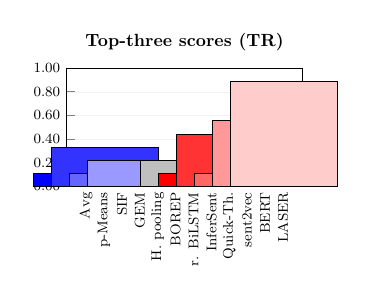
\begin{tikzpicture}[scale=0.75,every node/.style={scale=0.85}]
	\begin{axis}[
    		title=\textbf{Top-three scores (TR)},
		scale only axis,
		clip=false,
		separate axis lines,
		xtick={1,2,3,4,5,6,7,8,9,10,11,12},
        	x tick style={draw=none},
        	xticklabels={Avg,p-Means,SIF,GEM,H. pooling,BOREP,r. BiLSTM,InferSent,Quick-Th.,sent2vec,BERT,LASER},
		width=4cm,height=2cm,
		tick label style={font=\footnotesize},
		xticklabel style={rotate=90},
		ymajorgrids,
    		grid style={line width=.1pt, draw=gray!10},
		ymin=0,ymax=1,
		every axis plot/.append style={
          		ybar,
          		bar width=6.0,
          		bar shift=0.5pt,
			fill
		},
		scaled y ticks=false,
		y tick label style={
        		/pgf/number format/.cd,
            		fixed,
            		fixed zerofill,
            		precision=2,
        		/tikz/.cd
    		}
	]

		\addplot[draw=black,fill=blue] coordinates {(1,0.11)};
     	 	\addplot[draw=black,fill=blue!80] coordinates {(2,0.33)};
      		\addplot[draw=black,fill=blue!60] coordinates {(3,0.11)};
      		\addplot[draw=black,fill=blue!40] coordinates {(4,0.22)};
		\addplot[draw=black,fill=blue!20] coordinates {(5,0.00)};
     	 	\addplot[draw=black,fill=gray] coordinates {(6,0.00)};
      		\addplot[draw=black,fill=lightgray] coordinates {(7,0.22)};
      		\addplot[draw=black,fill=red] coordinates {(8,0.11)};
     	 	\addplot[draw=black,fill=red!80] coordinates {(9,0.44)};
      		\addplot[draw=black,fill=red!60] coordinates {(10,0.11)};
      		\addplot[draw=black,fill=red!40] coordinates {(11,0.56)};
		\addplot[draw=black,fill=red!20] coordinates {(12,0.89)};
	\end{axis}
\end{tikzpicture}
\end{minipage}
\hfill
\begin{minipage}[c]{0.30\textwidth}
\end{minipage}
\hfill
\begin{minipage}[c]{0.30\textwidth}
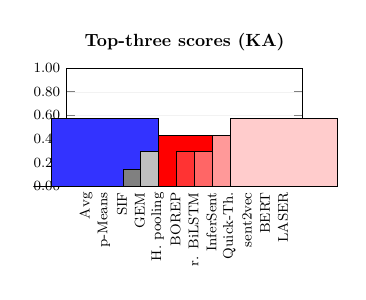
\begin{tikzpicture}[scale=0.75,every node/.style={scale=0.85}]
	\begin{axis}[
    		title=\textbf{Top-three scores (KA)},
		scale only axis,
		clip=false,
		separate axis lines,
		xtick={1,2,3,4,5,6,7,8,9,10,11,12},
        	x tick style={draw=none},
        	xticklabels={Avg,p-Means,SIF,GEM,H. pooling,BOREP,r. BiLSTM,InferSent,Quick-Th.,sent2vec,BERT,LASER},
		width=4cm,height=2cm,
		tick label style={font=\footnotesize},
		xticklabel style={rotate=90},
		ymajorgrids,
    		grid style={line width=.1pt, draw=gray!10},
		ymin=0,ymax=1,
		every axis plot/.append style={
          		ybar,
          		bar width=6.0,
          		bar shift=0.5pt,
			fill
		},
		scaled y ticks=false,
		y tick label style={
        		/pgf/number format/.cd,
            		fixed,
            		fixed zerofill,
            		precision=2,
        		/tikz/.cd
    		}
	]

		\addplot[draw=black,fill=blue] coordinates {(1,0.00)};
     	 	\addplot[draw=black,fill=blue!80] coordinates {(2,0.57)};
      		\addplot[draw=black,fill=blue!60] coordinates {(3,0.00)};
      		\addplot[draw=black,fill=blue!40] coordinates {(4,0.00)};
		\addplot[draw=black,fill=blue!20] coordinates {(5,0.00)};
     	 	\addplot[draw=black,fill=gray] coordinates {(6,0.14)};
      		\addplot[draw=black,fill=lightgray] coordinates {(7,0.29)};
      		\addplot[draw=black,fill=red] coordinates {(8,0.43)};
     	 	\addplot[draw=black,fill=red!80] coordinates {(9,0.29)};
      		\addplot[draw=black,fill=red!60] coordinates {(10,0.29)};
      		\addplot[draw=black,fill=red!40] coordinates {(11,0.43)};
		\addplot[draw=black,fill=red!20] coordinates {(12,0.57)};
	\end{axis}
\end{tikzpicture}
\end{minipage}
\end{figure}